\section{Use cases}
To get an overview of the system functionality from a user's perspective, the team applied \glspl{usecase}, which is a technique to help developers identify what functionality that should be implemented, and possible errors that might occur in the system.

The primary actors in our system is the user of the Android application. A use case diagram of the final version of the system is shown in figure~\ref{fig:usecase}.

Functionality that was initially included in the requirement specifictaion, but later left out, is discussed in chapter~\ref{sec:further}. 
\todo{her kan vi kanskje også nevne lista med frozen requirements i appendix B? Eller skal vi droppe appendix B helt?} For an overview of all textual use cases, see Appendix~\ref{sec:textUseCase}.\\

\begin{figure}[H]
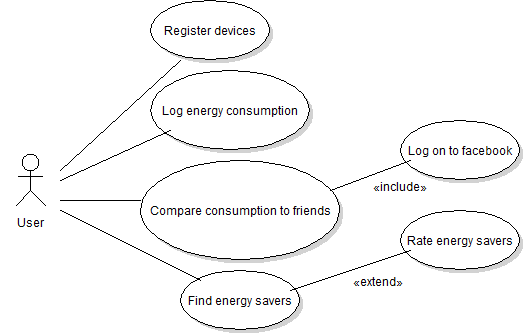
\includegraphics[width=\textwidth]{ch/specification/fig/currentUsecase.png}
\caption{Use case diagram for the entire system.}
\label{fig:usecase}
\end{figure}
